\documentclass[]{article}
\usepackage{lmodern}
\usepackage{amssymb,amsmath}
\usepackage{ifxetex,ifluatex}
\usepackage{fixltx2e} % provides \textsubscript
\ifnum 0\ifxetex 1\fi\ifluatex 1\fi=0 % if pdftex
  \usepackage[T1]{fontenc}
  \usepackage[utf8]{inputenc}
\else % if luatex or xelatex
  \ifxetex
    \usepackage{mathspec}
  \else
    \usepackage{fontspec}
  \fi
  \defaultfontfeatures{Ligatures=TeX,Scale=MatchLowercase}
\fi
% use upquote if available, for straight quotes in verbatim environments
\IfFileExists{upquote.sty}{\usepackage{upquote}}{}
% use microtype if available
\IfFileExists{microtype.sty}{%
\usepackage{microtype}
\UseMicrotypeSet[protrusion]{basicmath} % disable protrusion for tt fonts
}{}
\usepackage[margin=1in]{geometry}
\usepackage{hyperref}
\hypersetup{unicode=true,
            pdftitle={Introduction to mlr3},
            pdfborder={0 0 0},
            breaklinks=true}
\urlstyle{same}  % don't use monospace font for urls
\usepackage{color}
\usepackage{fancyvrb}
\newcommand{\VerbBar}{|}
\newcommand{\VERB}{\Verb[commandchars=\\\{\}]}
\DefineVerbatimEnvironment{Highlighting}{Verbatim}{commandchars=\\\{\}}
% Add ',fontsize=\small' for more characters per line
\usepackage{framed}
\definecolor{shadecolor}{RGB}{248,248,248}
\newenvironment{Shaded}{\begin{snugshade}}{\end{snugshade}}
\newcommand{\AlertTok}[1]{\textcolor[rgb]{0.94,0.16,0.16}{#1}}
\newcommand{\AnnotationTok}[1]{\textcolor[rgb]{0.56,0.35,0.01}{\textbf{\textit{#1}}}}
\newcommand{\AttributeTok}[1]{\textcolor[rgb]{0.77,0.63,0.00}{#1}}
\newcommand{\BaseNTok}[1]{\textcolor[rgb]{0.00,0.00,0.81}{#1}}
\newcommand{\BuiltInTok}[1]{#1}
\newcommand{\CharTok}[1]{\textcolor[rgb]{0.31,0.60,0.02}{#1}}
\newcommand{\CommentTok}[1]{\textcolor[rgb]{0.56,0.35,0.01}{\textit{#1}}}
\newcommand{\CommentVarTok}[1]{\textcolor[rgb]{0.56,0.35,0.01}{\textbf{\textit{#1}}}}
\newcommand{\ConstantTok}[1]{\textcolor[rgb]{0.00,0.00,0.00}{#1}}
\newcommand{\ControlFlowTok}[1]{\textcolor[rgb]{0.13,0.29,0.53}{\textbf{#1}}}
\newcommand{\DataTypeTok}[1]{\textcolor[rgb]{0.13,0.29,0.53}{#1}}
\newcommand{\DecValTok}[1]{\textcolor[rgb]{0.00,0.00,0.81}{#1}}
\newcommand{\DocumentationTok}[1]{\textcolor[rgb]{0.56,0.35,0.01}{\textbf{\textit{#1}}}}
\newcommand{\ErrorTok}[1]{\textcolor[rgb]{0.64,0.00,0.00}{\textbf{#1}}}
\newcommand{\ExtensionTok}[1]{#1}
\newcommand{\FloatTok}[1]{\textcolor[rgb]{0.00,0.00,0.81}{#1}}
\newcommand{\FunctionTok}[1]{\textcolor[rgb]{0.00,0.00,0.00}{#1}}
\newcommand{\ImportTok}[1]{#1}
\newcommand{\InformationTok}[1]{\textcolor[rgb]{0.56,0.35,0.01}{\textbf{\textit{#1}}}}
\newcommand{\KeywordTok}[1]{\textcolor[rgb]{0.13,0.29,0.53}{\textbf{#1}}}
\newcommand{\NormalTok}[1]{#1}
\newcommand{\OperatorTok}[1]{\textcolor[rgb]{0.81,0.36,0.00}{\textbf{#1}}}
\newcommand{\OtherTok}[1]{\textcolor[rgb]{0.56,0.35,0.01}{#1}}
\newcommand{\PreprocessorTok}[1]{\textcolor[rgb]{0.56,0.35,0.01}{\textit{#1}}}
\newcommand{\RegionMarkerTok}[1]{#1}
\newcommand{\SpecialCharTok}[1]{\textcolor[rgb]{0.00,0.00,0.00}{#1}}
\newcommand{\SpecialStringTok}[1]{\textcolor[rgb]{0.31,0.60,0.02}{#1}}
\newcommand{\StringTok}[1]{\textcolor[rgb]{0.31,0.60,0.02}{#1}}
\newcommand{\VariableTok}[1]{\textcolor[rgb]{0.00,0.00,0.00}{#1}}
\newcommand{\VerbatimStringTok}[1]{\textcolor[rgb]{0.31,0.60,0.02}{#1}}
\newcommand{\WarningTok}[1]{\textcolor[rgb]{0.56,0.35,0.01}{\textbf{\textit{#1}}}}
\usepackage{longtable,booktabs}
\usepackage{graphicx,grffile}
\makeatletter
\def\maxwidth{\ifdim\Gin@nat@width>\linewidth\linewidth\else\Gin@nat@width\fi}
\def\maxheight{\ifdim\Gin@nat@height>\textheight\textheight\else\Gin@nat@height\fi}
\makeatother
% Scale images if necessary, so that they will not overflow the page
% margins by default, and it is still possible to overwrite the defaults
% using explicit options in \includegraphics[width, height, ...]{}
\setkeys{Gin}{width=\maxwidth,height=\maxheight,keepaspectratio}
\IfFileExists{parskip.sty}{%
\usepackage{parskip}
}{% else
\setlength{\parindent}{0pt}
\setlength{\parskip}{6pt plus 2pt minus 1pt}
}
\setlength{\emergencystretch}{3em}  % prevent overfull lines
\providecommand{\tightlist}{%
  \setlength{\itemsep}{0pt}\setlength{\parskip}{0pt}}
\setcounter{secnumdepth}{0}
% Redefines (sub)paragraphs to behave more like sections
\ifx\paragraph\undefined\else
\let\oldparagraph\paragraph
\renewcommand{\paragraph}[1]{\oldparagraph{#1}\mbox{}}
\fi
\ifx\subparagraph\undefined\else
\let\oldsubparagraph\subparagraph
\renewcommand{\subparagraph}[1]{\oldsubparagraph{#1}\mbox{}}
\fi

%%% Use protect on footnotes to avoid problems with footnotes in titles
\let\rmarkdownfootnote\footnote%
\def\footnote{\protect\rmarkdownfootnote}

%%% Change title format to be more compact
\usepackage{titling}

% Create subtitle command for use in maketitle
\providecommand{\subtitle}[1]{
  \posttitle{
    \begin{center}\large#1\end{center}
    }
}

\setlength{\droptitle}{-2em}

  \title{Introduction to mlr3}
    \pretitle{\vspace{\droptitle}\centering\huge}
  \posttitle{\par}
    \author{}
    \preauthor{}\postauthor{}
    \date{}
    \predate{}\postdate{}
  

\begin{document}
\maketitle

{
\setcounter{tocdepth}{2}
\tableofcontents
}
\hypertarget{intro}{%
\section{Intro}\label{intro}}

\textbf{mlr3} is a machine learning framework for R. Together with other
packages from the same developers, mostly following the naming scheme
"mlr3\_\_\_", it offers functionality around developing, tuning, and
evaluating machine learning workflows.

We will walk through this tutorial interactively. The text is kept short
to be followed in real time. There are links to the
\protect\hyperlink{appendix}{Appendix} for further information that you
can read in your spare time.

\hypertarget{prerequisites}{%
\section{Prerequisites}\label{prerequisites}}

Ensure all packages used in this tutorial are installed. This includes
packages from the \texttt{mlr3} family, as well as other tools for data
handling, cleaning and visualisation which we are going to use.
\protect\hyperlink{packages}{Appendix for more info about packages}

\begin{Shaded}
\begin{Highlighting}[]
\CommentTok{# install from CRAN}
\NormalTok{packages_cran =}\StringTok{ }\KeywordTok{c}\NormalTok{(}
    \StringTok{"remotes"}\NormalTok{, }\StringTok{"magrittr"}\NormalTok{, }\StringTok{"data.table"}\NormalTok{, }\StringTok{"ggplot2"}\NormalTok{, }\StringTok{"skimr"}\NormalTok{, }\StringTok{"DataExplorer"}\NormalTok{,}
    \StringTok{"OpenML"}\NormalTok{, }\StringTok{"rpart.plot"}\NormalTok{, }\StringTok{"precrec"}\NormalTok{,}
    \StringTok{"glmnet"}\NormalTok{, }\StringTok{"kknn"}\NormalTok{, }\StringTok{"MASS"}\NormalTok{, }\StringTok{"ranger"}\NormalTok{, }\StringTok{"xgboost"}\NormalTok{, }\StringTok{"e1071"}\NormalTok{,}
    \StringTok{"future"}\NormalTok{, }\StringTok{"future.apply"}\NormalTok{,}
    \StringTok{"mlr3misc"}\NormalTok{, }\StringTok{"paradox"}\NormalTok{, }\StringTok{"mlr3"}\NormalTok{, }\StringTok{"mlr3filter"}\NormalTok{, }\StringTok{"mlr3learners"}\NormalTok{)}
\CommentTok{# install things from GitHub that are not yet on CRAN}
\NormalTok{packages_gith =}\StringTok{ }\KeywordTok{c}\NormalTok{(}
    \StringTok{"mlr-org/mlr3tuning"}\NormalTok{, }\StringTok{"mlr-org/mlr3pipelines"}\NormalTok{, }\StringTok{"mlr-org/mlr3viz"}\NormalTok{)}
\NormalTok{to_install =}\StringTok{ }\KeywordTok{setdiff}\NormalTok{(packages_cran, }\KeywordTok{installed.packages}\NormalTok{()[,}\StringTok{"Package"}\NormalTok{])}
\ControlFlowTok{if}\NormalTok{ (}\KeywordTok{length}\NormalTok{(to_install)) }\KeywordTok{install.packages}\NormalTok{(to_install)}
\KeywordTok{lapply}\NormalTok{(packages_gith, remotes}\OperatorTok{::}\NormalTok{install_github)}
\end{Highlighting}
\end{Shaded}

Load the packages we are going to use:

\begin{Shaded}
\begin{Highlighting}[]
\KeywordTok{library}\NormalTok{(}\StringTok{"data.table"}\NormalTok{)}
\KeywordTok{library}\NormalTok{(}\StringTok{"magrittr"}\NormalTok{)}
\KeywordTok{library}\NormalTok{(}\StringTok{"mlr3"}\NormalTok{)}
\KeywordTok{library}\NormalTok{(}\StringTok{"mlr3learners"}\NormalTok{)}
\KeywordTok{library}\NormalTok{(}\StringTok{"ggplot2"}\NormalTok{)}
\KeywordTok{theme_set}\NormalTok{(}\KeywordTok{theme_light}\NormalTok{())}
\end{Highlighting}
\end{Shaded}

\hypertarget{machine-learning-use-case-german-credit-data}{%
\section{Machine Learning Use Case: German Credit
Data}\label{machine-learning-use-case-german-credit-data}}

\begin{itemize}
\tightlist
\item
  The German credit data is a research data set of the University of
  Hamburg from 1994 donated by Prof.~Hans Hoffman.
\item
  Description (and manual download) can be found at the
  \href{https://archive.ics.uci.edu/ml/datasets/Statlog+\%28German+Credit+Data\%29}{UCI
  repository}.
\item
  Goal: Classify people by their credit risk (\textbf{good} or
  \textbf{bad}) using 20 features.
\end{itemize}

\hypertarget{importing-the-data}{%
\subsection{Importing the data}\label{importing-the-data}}

We use \href{https://www.openml.org}{OpenML}
(\href{https://cran.r-project.org/package=OpenML}{R-Package}) to
download the data set in a machine-readable format and convert it into a
\texttt{data.table}:

\begin{Shaded}
\begin{Highlighting}[]
\CommentTok{# load the data set (id 31) from OpenML Library and}
\CommentTok{# convert the OpenML object to a regular data.table.}
\CommentTok{# The encapsulate() is important.}
\NormalTok{credit =}\StringTok{ }\NormalTok{mlr3misc}\OperatorTok{::}\KeywordTok{encapsulate}\NormalTok{(}\StringTok{"callr"}\NormalTok{, }\ControlFlowTok{function}\NormalTok{() \{}
\NormalTok{  data.table}\OperatorTok{::}\KeywordTok{as.data.table}\NormalTok{(OpenML}\OperatorTok{::}\KeywordTok{getOMLDataSet}\NormalTok{(}\DataTypeTok{data.id =} \DecValTok{31}\NormalTok{))}
\NormalTok{\})}\OperatorTok{$}\NormalTok{result}
\end{Highlighting}
\end{Shaded}

\hypertarget{exploring-the-data}{%
\subsection{Exploring the Data}\label{exploring-the-data}}

\begin{itemize}
\tightlist
\item
  We have a look at the data set before we start modeling.
\item
  The \texttt{str()} and \texttt{summary()} functions gives an overview
  of features and their type.
\item
  The \texttt{skimr} package gives more readable summaries.
\item
  The \texttt{DataExplorer} package lets us visualise numeric
  (\texttt{plot\_histogram()}) and categorical (\texttt{plot\_bar()})
  data, as well as data relationships.
\item
  Basic things to watch out for:

  \begin{itemize}
  \tightlist
  \item
    Skewed distributions
  \item
    Missing values
  \item
    Empty / rare factor variables
  \item
    Strongly correlating features (``multicollinearity'')
  \end{itemize}
\end{itemize}

\begin{Shaded}
\begin{Highlighting}[]
\KeywordTok{str}\NormalTok{(credit)}
\CommentTok{#> Classes 'data.table' and 'data.frame':   1000 obs. of  21 variables:}
\CommentTok{#>  $ checking_status       : Factor w/ 4 levels "<0","0<=X<200",..: 1 2 4 1 1 4 4 2 4 2 ...}
\CommentTok{#>  $ duration              : num  6 48 12 42 24 36 24 36 12 30 ...}
\CommentTok{#>  $ credit_history        : Factor w/ 5 levels "no credits/all paid",..: 5 3 5 3 4 3 3 3 3 5 ...}
\CommentTok{#>  $ purpose               : Factor w/ 11 levels "new car","used car",..: 4 4 7 3 1 7 3 2 4 1 ...}
\CommentTok{#>  $ credit_amount         : num  1169 5951 2096 7882 4870 ...}
\CommentTok{#>  $ savings_status        : Factor w/ 5 levels "<100","100<=X<500",..: 5 1 1 1 1 5 3 1 4 1 ...}
\CommentTok{#>  $ employment            : Factor w/ 5 levels "unemployed","<1",..: 5 3 4 4 3 3 5 3 4 1 ...}
\CommentTok{#>  $ installment_commitment: num  4 2 2 2 3 2 3 2 2 4 ...}
\CommentTok{#>  $ personal_status       : Factor w/ 5 levels "male div/sep",..: 3 2 3 3 3 3 3 3 1 4 ...}
\CommentTok{#>  $ other_parties         : Factor w/ 3 levels "none","co applicant",..: 1 1 1 3 1 1 1 1 1 1 ...}
\CommentTok{#>  $ residence_since       : num  4 2 3 4 4 4 4 2 4 2 ...}
\CommentTok{#>  $ property_magnitude    : Factor w/ 4 levels "real estate",..: 1 1 1 2 4 4 2 3 1 3 ...}
\CommentTok{#>  $ age                   : num  67 22 49 45 53 35 53 35 61 28 ...}
\CommentTok{#>  $ other_payment_plans   : Factor w/ 3 levels "bank","stores",..: 3 3 3 3 3 3 3 3 3 3 ...}
\CommentTok{#>  $ housing               : Factor w/ 3 levels "rent","own","for free": 2 2 2 3 3 3 2 1 2 2 ...}
\CommentTok{#>  $ existing_credits      : num  2 1 1 1 2 1 1 1 1 2 ...}
\CommentTok{#>  $ job                   : Factor w/ 4 levels "unemp/unskilled non res",..: 3 3 2 3 3 2 3 4 2 4 ...}
\CommentTok{#>  $ num_dependents        : num  1 1 2 2 2 2 1 1 1 1 ...}
\CommentTok{#>  $ own_telephone         : Factor w/ 2 levels "none","yes": 2 1 1 1 1 2 1 2 1 1 ...}
\CommentTok{#>  $ foreign_worker        : Factor w/ 2 levels "yes","no": 1 1 1 1 1 1 1 1 1 1 ...}
\CommentTok{#>  $ class                 : Factor w/ 2 levels "good","bad": 1 2 1 1 2 1 1 1 1 2 ...}
\CommentTok{#>  - attr(*, ".internal.selfref")=<externalptr>}
\end{Highlighting}
\end{Shaded}

\begin{Shaded}
\begin{Highlighting}[]
\KeywordTok{summary}\NormalTok{(credit)}
\CommentTok{#>     checking_status    duration                           credit_history}
\CommentTok{#>  <0         :274    Min.   : 4.0   no credits/all paid           : 40   }
\CommentTok{#>  0<=X<200   :269    1st Qu.:12.0   all paid                      : 49   }
\CommentTok{#>  >=200      : 63    Median :18.0   existing paid                 :530   }
\CommentTok{#>  no checking:394    Mean   :20.9   delayed previously            : 88   }
\CommentTok{#>                     3rd Qu.:24.0   critical/other existing credit:293   }
\CommentTok{#>                     Max.   :72.0                                        }
\CommentTok{#>                                                                         }
\CommentTok{#>                 purpose    credit_amount            savings_status      employment }
\CommentTok{#>  radio/tv           :280   Min.   :  250   <100            :603    unemployed: 62  }
\CommentTok{#>  new car            :234   1st Qu.: 1366   100<=X<500      :103    <1        :172  }
\CommentTok{#>  furniture/equipment:181   Median : 2320   500<=X<1000     : 63    1<=X<4    :339  }
\CommentTok{#>  used car           :103   Mean   : 3271   >=1000          : 48    4<=X<7    :174  }
\CommentTok{#>  business           : 97   3rd Qu.: 3972   no known savings:183    >=7       :253  }
\CommentTok{#>  education          : 50   Max.   :18424                                           }
\CommentTok{#>  (Other)            : 55                                                           }
\CommentTok{#>  installment_commitment           personal_status      other_parties residence_since}
\CommentTok{#>  Min.   :1.000          male div/sep      : 50    none        :907   Min.   :1.000  }
\CommentTok{#>  1st Qu.:2.000          female div/dep/mar:310    co applicant: 41   1st Qu.:2.000  }
\CommentTok{#>  Median :3.000          male single       :548    guarantor   : 52   Median :3.000  }
\CommentTok{#>  Mean   :2.973          male mar/wid      : 92                       Mean   :2.845  }
\CommentTok{#>  3rd Qu.:4.000          female single     :  0                       3rd Qu.:4.000  }
\CommentTok{#>  Max.   :4.000                                                       Max.   :4.000  }
\CommentTok{#>                                                                                     }
\CommentTok{#>          property_magnitude      age        other_payment_plans     housing   }
\CommentTok{#>  real estate      :282      Min.   :19.00   bank  :139          rent    :179  }
\CommentTok{#>  life insurance   :232      1st Qu.:27.00   stores: 47          own     :713  }
\CommentTok{#>  car              :332      Median :33.00   none  :814          for free:108  }
\CommentTok{#>  no known property:154      Mean   :35.55                                     }
\CommentTok{#>                             3rd Qu.:42.00                                     }
\CommentTok{#>                             Max.   :75.00                                     }
\CommentTok{#>                                                                               }
\CommentTok{#>  existing_credits                        job      num_dependents  own_telephone}
\CommentTok{#>  Min.   :1.000    unemp/unskilled non res  : 22   Min.   :1.000   none:596     }
\CommentTok{#>  1st Qu.:1.000    unskilled resident       :200   1st Qu.:1.000   yes :404     }
\CommentTok{#>  Median :1.000    skilled                  :630   Median :1.000                }
\CommentTok{#>  Mean   :1.407    high qualif/self emp/mgmt:148   Mean   :1.155                }
\CommentTok{#>  3rd Qu.:2.000                                    3rd Qu.:1.000                }
\CommentTok{#>  Max.   :4.000                                    Max.   :2.000                }
\CommentTok{#>                                                                                }
\CommentTok{#>  foreign_worker  class    }
\CommentTok{#>  yes:963        good:700  }
\CommentTok{#>  no : 37        bad :300  }
\CommentTok{#>                           }
\CommentTok{#>                           }
\CommentTok{#>                           }
\CommentTok{#>                           }
\CommentTok{#> }
\end{Highlighting}
\end{Shaded}

\begin{Shaded}
\begin{Highlighting}[]
\NormalTok{skimr}\OperatorTok{::}\KeywordTok{skim}\NormalTok{(credit)}
\CommentTok{#> Skim summary statistics}
\CommentTok{#>  n obs: 1000 }
\CommentTok{#>  n variables: 21 }
\CommentTok{#> }
\CommentTok{#> -- Variable type:factor ----------------------------------------------------------------------------------}
\CommentTok{#>             variable missing complete    n n_unique}
\CommentTok{#>      checking_status       0     1000 1000        4}
\CommentTok{#>                class       0     1000 1000        2}
\CommentTok{#>       credit_history       0     1000 1000        5}
\CommentTok{#>           employment       0     1000 1000        5}
\CommentTok{#>       foreign_worker       0     1000 1000        2}
\CommentTok{#>              housing       0     1000 1000        3}
\CommentTok{#>                  job       0     1000 1000        4}
\CommentTok{#>        other_parties       0     1000 1000        3}
\CommentTok{#>  other_payment_plans       0     1000 1000        3}
\CommentTok{#>        own_telephone       0     1000 1000        2}
\CommentTok{#>      personal_status       0     1000 1000        4}
\CommentTok{#>   property_magnitude       0     1000 1000        4}
\CommentTok{#>              purpose       0     1000 1000       10}
\CommentTok{#>       savings_status       0     1000 1000        5}
\CommentTok{#>                              top_counts ordered}
\CommentTok{#>    no : 394, <0: 274, 0<=: 269, >=2: 63   FALSE}
\CommentTok{#>               goo: 700, bad: 300, NA: 0   FALSE}
\CommentTok{#>    exi: 530, cri: 293, del: 88, all: 49   FALSE}
\CommentTok{#>   1<=: 339, >=7: 253, 4<=: 174, <1: 172   FALSE}
\CommentTok{#>                 yes: 963, no: 37, NA: 0   FALSE}
\CommentTok{#>     own: 713, ren: 179, for: 108, NA: 0   FALSE}
\CommentTok{#>   ski: 630, uns: 200, hig: 148, une: 22   FALSE}
\CommentTok{#>       non: 907, gua: 52, co : 41, NA: 0   FALSE}
\CommentTok{#>      non: 814, ban: 139, sto: 47, NA: 0   FALSE}
\CommentTok{#>               non: 596, yes: 404, NA: 0   FALSE}
\CommentTok{#>    mal: 548, fem: 310, mal: 92, mal: 50   FALSE}
\CommentTok{#>  car: 332, rea: 282, lif: 232, no : 154   FALSE}
\CommentTok{#>  rad: 280, new: 234, fur: 181, use: 103   FALSE}
\CommentTok{#>   <10: 603, no : 183, 100: 103, 500: 63   FALSE}
\CommentTok{#> }
\CommentTok{#> -- Variable type:numeric ---------------------------------------------------------------------------------}
\CommentTok{#>                variable missing complete    n    mean      sd  p0    p25    p50     p75}
\CommentTok{#>                     age       0     1000 1000   35.55   11.38  19   27     33     42   }
\CommentTok{#>           credit_amount       0     1000 1000 3271.26 2822.74 250 1365.5 2319.5 3972.25}
\CommentTok{#>                duration       0     1000 1000   20.9    12.06   4   12     18     24   }
\CommentTok{#>        existing_credits       0     1000 1000    1.41    0.58   1    1      1      2   }
\CommentTok{#>  installment_commitment       0     1000 1000    2.97    1.12   1    2      3      4   }
\CommentTok{#>          num_dependents       0     1000 1000    1.16    0.36   1    1      1      1   }
\CommentTok{#>         residence_since       0     1000 1000    2.85    1.1    1    2      3      4   }
\CommentTok{#>   p100     hist}
\CommentTok{#>     75 ▇▇▆▃▂▁▁▁}
\CommentTok{#>  18424 ▇▃▂▁▁▁▁▁}
\CommentTok{#>     72 ▇▅▅▃▁▁▁▁}
\CommentTok{#>      4 ▇▁▅▁▁▁▁▁}
\CommentTok{#>      4 ▂▁▃▁▁▂▁▇}
\CommentTok{#>      2 ▇▁▁▁▁▁▁▂}
\CommentTok{#>      4 ▂▁▆▁▁▃▁▇}
\end{Highlighting}
\end{Shaded}

\begin{Shaded}
\begin{Highlighting}[]
\NormalTok{DataExplorer}\OperatorTok{::}\KeywordTok{plot_histogram}\NormalTok{(credit)}
\end{Highlighting}
\end{Shaded}

\includegraphics{04e-mlr_intro_files/figure-latex/unnamed-chunk-8-1.pdf}

\begin{Shaded}
\begin{Highlighting}[]
\NormalTok{DataExplorer}\OperatorTok{::}\KeywordTok{plot_bar}\NormalTok{(credit)}
\end{Highlighting}
\end{Shaded}

\includegraphics{04e-mlr_intro_files/figure-latex/unnamed-chunk-9-1.pdf}
\includegraphics{04e-mlr_intro_files/figure-latex/unnamed-chunk-9-2.pdf}

\begin{Shaded}
\begin{Highlighting}[]
\NormalTok{DataExplorer}\OperatorTok{::}\KeywordTok{split_columns}\NormalTok{(credit) }\OperatorTok
\StringTok{  }\NormalTok{DataExplorer}\OperatorTok{::}\KeywordTok{plot_correlation}\NormalTok{(continuous)}
\end{Highlighting}
\end{Shaded}

\includegraphics{04e-mlr_intro_files/figure-latex/unnamed-chunk-10-1.pdf}

\begin{Shaded}
\begin{Highlighting}[]
\NormalTok{DataExplorer}\OperatorTok{::}\KeywordTok{plot_boxplot}\NormalTok{(credit, }\DataTypeTok{by =} \StringTok{"class"}\NormalTok{)}
\end{Highlighting}
\end{Shaded}

\includegraphics{04e-mlr_intro_files/figure-latex/unnamed-chunk-11-1.pdf}

\begin{itemize}
\tightlist
\item
  We have empty factor levels, so we drop them:
\end{itemize}

\begin{Shaded}
\begin{Highlighting}[]
\NormalTok{credit }\OperatorTok\StringTok{ }\KeywordTok{droplevels}\NormalTok{()}
\end{Highlighting}
\end{Shaded}

\hypertarget{modeling}{%
\section{Modeling}\label{modeling}}

Considering how we are going to tackle the problem relates closely to
what \texttt{mlr3} entities we will use.

\begin{itemize}
\tightlist
\item
  What is the problem we are trying to solve?

  \begin{itemize}
  \tightlist
  \item
    i.e.~what \textbf{Task} do we use?
  \item
    Binary classification.
  \item
    \(\Rightarrow\) We use \texttt{TaskClassif}.
  \end{itemize}
\item
  What are appropriate learning algorithms?

  \begin{itemize}
  \tightlist
  \item
    i.e.~what \textbf{Learner} do we use?
  \item
    Logistic regression, CART, Random Forest
  \item
    \(\Rightarrow\) \texttt{lrn("classif.log\_reg")},
    \texttt{lrn("classif.rpart")}, \texttt{lrn("classif.ranger")}
  \end{itemize}
\item
  How do we evaluate ``good'' performance? \(\Rightarrow\) Depends on
  many things! Cost of false positive vs.~false negative, legal
  requirements, \ldots{}

  \begin{itemize}
  \tightlist
  \item
    i.e.~what \textbf{Measure} do we use?
  \item
    We start with misclassification error (simle!) and will also
    consider AUC.
  \item
    \(\Rightarrow\) \texttt{msr("classif.ce")},
    \texttt{msr("classif.auc")}
  \end{itemize}
\end{itemize}

\hypertarget{task-definition}{%
\subsection{Task Definition}\label{task-definition}}

\begin{itemize}
\tightlist
\item
  We need to consider what the name of the target variable is:
  \texttt{"class"}.
\end{itemize}

\begin{Shaded}
\begin{Highlighting}[]
\NormalTok{task =}\StringTok{ }\NormalTok{TaskClassif}\OperatorTok{$}\KeywordTok{new}\NormalTok{(}\StringTok{"GermanCredit"}\NormalTok{, credit, }\StringTok{"class"}\NormalTok{)}
\end{Highlighting}
\end{Shaded}

\hypertarget{model-fitting-logistic-regression}{%
\subsection{Model Fitting: Logistic
Regression}\label{model-fitting-logistic-regression}}

\begin{itemize}
\tightlist
\item
  Get the \texttt{Learner} from the database. It is provided by
  \texttt{mlr3learners} and uses R's \texttt{glm()} function.
\end{itemize}

\begin{Shaded}
\begin{Highlighting}[]
\NormalTok{learner_logreg =}\StringTok{ }\KeywordTok{lrn}\NormalTok{(}\StringTok{"classif.log_reg"}\NormalTok{)}
\end{Highlighting}
\end{Shaded}

\begin{itemize}
\tightlist
\item
  Model fitting is easy
\end{itemize}

\begin{Shaded}
\begin{Highlighting}[]
\NormalTok{learner_logreg}\OperatorTok{$}\KeywordTok{train}\NormalTok{(task)}
\end{Highlighting}
\end{Shaded}

\begin{itemize}
\tightlist
\item
  Inspecting the model. It is the result returned by \texttt{glm()} and
  can be inspected as such.
\end{itemize}

\begin{Shaded}
\begin{Highlighting}[]
\NormalTok{coefficients =}\StringTok{ }\NormalTok{learner_logreg}\OperatorTok{$}\NormalTok{model }\OperatorTok\StringTok{ }\KeywordTok{summary}\NormalTok{() }\OperatorTok
\StringTok{  }\KeywordTok{as.data.table}\NormalTok{(coefficients, }\DataTypeTok{keep.rownames =} \OtherTok{TRUE}\NormalTok{)}
\NormalTok{coefficients[}\KeywordTok{order}\NormalTok{(}\StringTok{`}\DataTypeTok{Pr(>|z|)}\StringTok{`}\NormalTok{)] }\OperatorTok\StringTok{ }\KeywordTok{head}\NormalTok{(}\DataTypeTok{n =} \DecValTok{10}\NormalTok{) }\OperatorTok\StringTok{ }\KeywordTok{print}\NormalTok{(}\DataTypeTok{digits =} \DecValTok{3}\NormalTok{)}
\CommentTok{#>                                               rn  Estimate Std. Error z value Pr(>|z|)}
\CommentTok{#>  1:                   checking_statusno checking -1.711888   2.32e-01   -7.37 1.66e-13}
\CommentTok{#>  2:                              purposeused car -1.666467   3.74e-01   -4.45 8.51e-06}
\CommentTok{#>  3:                       installment_commitment  0.330090   8.83e-02    3.74 1.85e-04}
\CommentTok{#>  4:                              purposeradio/tv -0.891583   2.47e-01   -3.61 3.08e-04}
\CommentTok{#>  5:               savings_statusno known savings -0.946689   2.62e-01   -3.61 3.10e-04}
\CommentTok{#>  6: credit_historycritical/other existing credit -1.435772   4.40e-01   -3.26 1.10e-03}
\CommentTok{#>  7:                   purposefurniture/equipment -0.791610   2.61e-01   -3.03 2.42e-03}
\CommentTok{#>  8:                                     duration  0.027863   9.30e-03    3.00 2.72e-03}
\CommentTok{#>  9:                                credit_amount  0.000128   4.44e-05    2.89 3.89e-03}
\CommentTok{#> 10:                      other_payment_plansnone -0.646329   2.39e-01   -2.70 6.87e-03}
\end{Highlighting}
\end{Shaded}

\hypertarget{model-fitting-decision-tree}{%
\subsection{Model Fitting: Decision
Tree}\label{model-fitting-decision-tree}}

\begin{itemize}
\tightlist
\item
  Same procedure as before
\item
  We fit a decision tree with depth 3 for nicer plots
\end{itemize}

\begin{Shaded}
\begin{Highlighting}[]
\NormalTok{learner_cart =}\StringTok{ }\KeywordTok{lrn}\NormalTok{(}\StringTok{"classif.rpart"}\NormalTok{, }\DataTypeTok{maxdepth =} \DecValTok{3}\NormalTok{)}
\NormalTok{learner_cart}\OperatorTok{$}\KeywordTok{train}\NormalTok{(task)}
\end{Highlighting}
\end{Shaded}

\begin{itemize}
\tightlist
\item
  The \texttt{rpart.plot} library gives expressive plots:
\end{itemize}

\begin{Shaded}
\begin{Highlighting}[]
\NormalTok{rpart.plot}\OperatorTok{::}\KeywordTok{rpart.plot}\NormalTok{(learner_cart}\OperatorTok{$}\NormalTok{model)}
\CommentTok{#> Warning: Bad 'data' field in model 'call' (expected a data.frame or a matrix).}
\CommentTok{#> To silence this warning:}
\CommentTok{#>     Call rpart.plot with roundint=FALSE,}
\CommentTok{#>     or rebuild the rpart model with model=TRUE.}
\end{Highlighting}
\end{Shaded}

\includegraphics{04e-mlr_intro_files/figure-latex/unnamed-chunk-19-1.pdf}

\hypertarget{model-fitting-random-forest}{%
\subsection{Model Fitting: Random
Forest}\label{model-fitting-random-forest}}

\begin{itemize}
\tightlist
\item
  Same procedure as before
\item
  We let the model store the variable importance
  (\texttt{importance\ =\ "impurity\_corrected"}) which we can inspect
  using \texttt{\$importance()}
\end{itemize}

\begin{Shaded}
\begin{Highlighting}[]
\NormalTok{learner_rf =}\StringTok{ }\KeywordTok{lrn}\NormalTok{(}\StringTok{"classif.ranger"}\NormalTok{, }\DataTypeTok{importance =} \StringTok{"impurity"}\NormalTok{)}
\NormalTok{learner_rf}\OperatorTok{$}\KeywordTok{train}\NormalTok{(task)}
\end{Highlighting}
\end{Shaded}

\begin{Shaded}
\begin{Highlighting}[]
\NormalTok{learner_rf}\OperatorTok{$}\KeywordTok{importance}\NormalTok{()}
\CommentTok{#>          credit_amount        checking_status                    age }
\CommentTok{#>              55.023916              47.062750              43.147626 }
\CommentTok{#>               duration                purpose         credit_history }
\CommentTok{#>              41.220088              25.116997              24.733077 }
\CommentTok{#>             employment         savings_status     property_magnitude }
\CommentTok{#>              21.368195              20.082949              18.941929 }
\CommentTok{#> installment_commitment        residence_since        personal_status }
\CommentTok{#>              17.410324              16.753125              15.301674 }
\CommentTok{#>                    job    other_payment_plans                housing }
\CommentTok{#>              13.312583              11.511337              10.598417 }
\CommentTok{#>       existing_credits          own_telephone          other_parties }
\CommentTok{#>               9.242539               8.207242               8.004813 }
\CommentTok{#>         num_dependents         foreign_worker }
\CommentTok{#>               5.778569               1.798239}
\end{Highlighting}
\end{Shaded}

\begin{itemize}
\tightlist
\item
  We convert the importance into a \texttt{data.table} so we can plot it
\end{itemize}

\begin{Shaded}
\begin{Highlighting}[]
\NormalTok{importance =}\StringTok{ }\KeywordTok{as.data.table}\NormalTok{(learner_rf}\OperatorTok{$}\KeywordTok{importance}\NormalTok{(), }\DataTypeTok{keep.rownames =} \OtherTok{TRUE}\NormalTok{)}
\KeywordTok{colnames}\NormalTok{(importance) =}\StringTok{ }\KeywordTok{c}\NormalTok{(}\StringTok{"Feature"}\NormalTok{, }\StringTok{"Importance"}\NormalTok{)}
\NormalTok{importance}
\CommentTok{#>                    Feature Importance}
\CommentTok{#>  1:          credit_amount  55.023916}
\CommentTok{#>  2:        checking_status  47.062750}
\CommentTok{#>  3:                    age  43.147626}
\CommentTok{#>  4:               duration  41.220088}
\CommentTok{#>  5:                purpose  25.116997}
\CommentTok{#>  6:         credit_history  24.733077}
\CommentTok{#>  7:             employment  21.368195}
\CommentTok{#>  8:         savings_status  20.082949}
\CommentTok{#>  9:     property_magnitude  18.941929}
\CommentTok{#> 10: installment_commitment  17.410324}
\CommentTok{#> 11:        residence_since  16.753125}
\CommentTok{#> 12:        personal_status  15.301674}
\CommentTok{#> 13:                    job  13.312583}
\CommentTok{#> 14:    other_payment_plans  11.511337}
\CommentTok{#> 15:                housing  10.598417}
\CommentTok{#> 16:       existing_credits   9.242539}
\CommentTok{#> 17:          own_telephone   8.207242}
\CommentTok{#> 18:          other_parties   8.004813}
\CommentTok{#> 19:         num_dependents   5.778569}
\CommentTok{#> 20:         foreign_worker   1.798239}
\KeywordTok{ggplot}\NormalTok{(importance, }\KeywordTok{aes}\NormalTok{(}\DataTypeTok{x =} \KeywordTok{reorder}\NormalTok{(Feature, Importance), }\DataTypeTok{y =}\NormalTok{ Importance)) }\OperatorTok{+}
\StringTok{  }\KeywordTok{geom_col}\NormalTok{() }\OperatorTok{+}\StringTok{ }\KeywordTok{coord_flip}\NormalTok{() }\OperatorTok{+}\StringTok{ }\KeywordTok{xlab}\NormalTok{(}\StringTok{""}\NormalTok{)}
\end{Highlighting}
\end{Shaded}

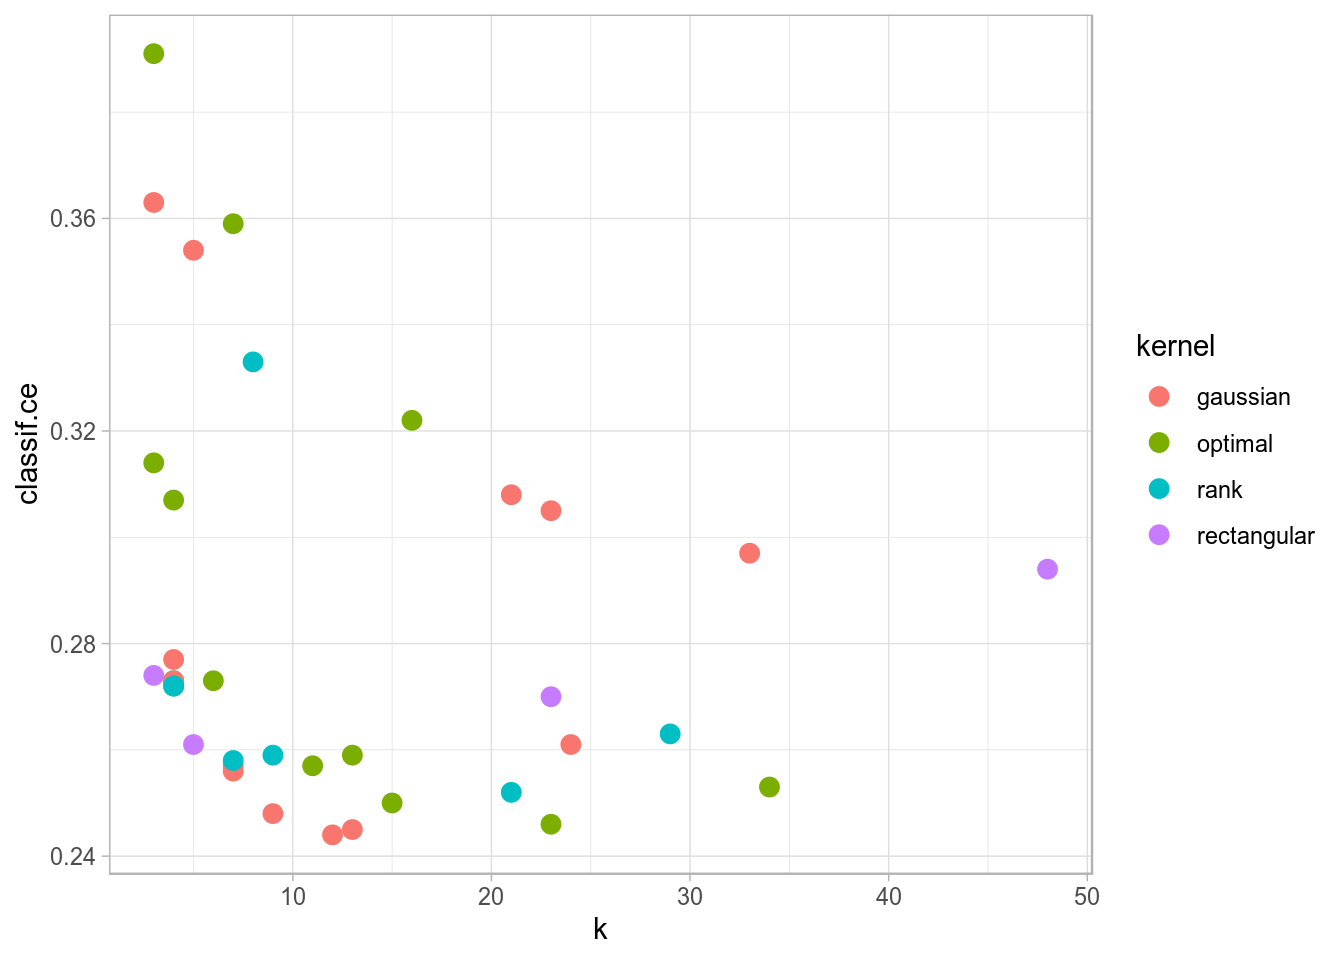
\includegraphics{04e-mlr_intro_files/figure-latex/unnamed-chunk-22-1.pdf}

\hypertarget{model-fitting-other-models}{%
\subsection{Model Fitting: Other
Models}\label{model-fitting-other-models}}

Feel free to experiment with other \texttt{Learner}s! There are many
\texttt{Learner}s defined in \texttt{mlr\_learners}. You need to load
the \texttt{mlr3learners} package to get access to most of them.

Use \texttt{?mlr\_learners\_xxx} or
\texttt{help(class(lrn("xxx")){[}1{]})} to see the help page, or use
\href{https://mlr3learners.mlr-org.com/reference/index.html}{the
internet}.

\begin{Shaded}
\begin{Highlighting}[]
\NormalTok{mlr_learners}
\CommentTok{#> <DictionaryLearner> with 21 stored values}
\CommentTok{#> Keys: classif.debug, classif.featureless, classif.glmnet, classif.kknn,}
\CommentTok{#>   classif.lda, classif.log_reg, classif.naive_bayes, classif.qda,}
\CommentTok{#>   classif.ranger, classif.rpart, classif.svm, classif.xgboost, regr.featureless,}
\CommentTok{#>   regr.glmnet, regr.kknn, regr.km, regr.lm, regr.ranger, regr.rpart, regr.svm,}
\CommentTok{#>   regr.xgboost}
\end{Highlighting}
\end{Shaded}

\hypertarget{prediction}{%
\section{Prediction}\label{prediction}}

\begin{itemize}
\tightlist
\item
  A model, once trained, can be used to predict outcomes from new data.
\item
  This new data needs to be loaded as a \texttt{Task} as well, then the
  \texttt{Learner}'s \texttt{\$predict()} function can be used.
\item
  We simulate new data by sampling from the credit data. No need to pay
  close attention what is going on here.
\end{itemize}

\begin{Shaded}
\begin{Highlighting}[]
\NormalTok{newdata =}\StringTok{ }\KeywordTok{as.data.table}\NormalTok{(}\KeywordTok{lapply}\NormalTok{(credit, sample, }\DataTypeTok{size =} \DecValTok{3}\NormalTok{, }\DataTypeTok{replace =} \OtherTok{TRUE}\NormalTok{))}
\CommentTok{# we need to set the 'class' column to 'NA', otherwise mlr3 thinks this is the}
\CommentTok{# actual outcome. This is desirable for performance evaluation, but not here.}
\NormalTok{newdata}\OperatorTok{$}\NormalTok{class[}\DecValTok{1}\OperatorTok{:}\DecValTok{3}\NormalTok{] =}\StringTok{ }\OtherTok{NA}
\end{Highlighting}
\end{Shaded}

\begin{Shaded}
\begin{Highlighting}[]
\NormalTok{new_task =}\StringTok{ }\NormalTok{TaskClassif}\OperatorTok{$}\KeywordTok{new}\NormalTok{(}\StringTok{"new_credit"}\NormalTok{, newdata, }\StringTok{"class"}\NormalTok{, }\DataTypeTok{positive =} \StringTok{"good"}\NormalTok{)}
\end{Highlighting}
\end{Shaded}

\begin{itemize}
\tightlist
\item
  Let's see what the models predict
\end{itemize}

\begin{Shaded}
\begin{Highlighting}[]
\NormalTok{learner_logreg}\OperatorTok{$}\KeywordTok{predict}\NormalTok{(new_task)}
\CommentTok{#> <PredictionClassif> for 3 observations:}
\CommentTok{#>  row_id truth response}
\CommentTok{#>       1  <NA>     good}
\CommentTok{#>       2  <NA>     good}
\CommentTok{#>       3  <NA>      bad}
\NormalTok{learner_cart}\OperatorTok{$}\KeywordTok{predict}\NormalTok{(new_task)}
\CommentTok{#> <PredictionClassif> for 3 observations:}
\CommentTok{#>  row_id truth response}
\CommentTok{#>       1  <NA>     good}
\CommentTok{#>       2  <NA>     good}
\CommentTok{#>       3  <NA>      bad}
\NormalTok{learner_rf}\OperatorTok{$}\KeywordTok{predict}\NormalTok{(new_task)}
\CommentTok{#> <PredictionClassif> for 3 observations:}
\CommentTok{#>  row_id truth response}
\CommentTok{#>       1  <NA>      bad}
\CommentTok{#>       2  <NA>     good}
\CommentTok{#>       3  <NA>     good}
\end{Highlighting}
\end{Shaded}

\begin{itemize}
\tightlist
\item
  They may disagree, but which do we trust most? We should do
  \protect\hyperlink{performance-evaluation}{Performance Evaluation} and
  \protect\hyperlink{performance-comparison-and-benchmarks}{benchmarks}!
\end{itemize}

\hypertarget{probability-prediction}{%
\subsection{Probability Prediction}\label{probability-prediction}}

\begin{itemize}
\tightlist
\item
  Learners may not only predict a class variable (``response''), but
  also their degree of ``belief'' / uncertainty in a given response.
\item
  We achieve this by setting the \texttt{\$predict\_type} slot to
  \texttt{"prob"}.
\item
  Sometimes this needs to be done \emph{before} the learner is trained.
\item
  Can alternatively construct with this:
  \texttt{lrn("classif.log\_reg",\ predict\_type\ =\ "prob")}
\end{itemize}

\begin{Shaded}
\begin{Highlighting}[]
\NormalTok{learner_logreg}\OperatorTok{$}\NormalTok{predict_type =}\StringTok{ "prob"}
\end{Highlighting}
\end{Shaded}

\begin{Shaded}
\begin{Highlighting}[]
\NormalTok{learner_logreg}\OperatorTok{$}\KeywordTok{predict}\NormalTok{(new_task)}
\CommentTok{#> <PredictionClassif> for 3 observations:}
\CommentTok{#>  row_id truth response prob.good  prob.bad}
\CommentTok{#>       1  <NA>     good 0.6877390 0.3122610}
\CommentTok{#>       2  <NA>     good 0.7727115 0.2272885}
\CommentTok{#>       3  <NA>      bad 0.4500287 0.5499713}
\end{Highlighting}
\end{Shaded}

\begin{itemize}
\tightlist
\item
  Careful when interpreting this as probabilities!
\end{itemize}

\hypertarget{performance-evaluation}{%
\section{Performance Evaluation}\label{performance-evaluation}}

\hypertarget{the-hard-way}{%
\subsection{The Hard way}\label{the-hard-way}}

To show what is happening behind the scenes we will do one round of
resampling ourselves 1. Decide on a train/test split.

\begin{Shaded}
\begin{Highlighting}[]
\NormalTok{train_set =}\StringTok{ }\KeywordTok{sample}\NormalTok{(}\KeywordTok{nrow}\NormalTok{(credit), }\DataTypeTok{size =} \KeywordTok{nrow}\NormalTok{(credit) }\OperatorTok{*}\StringTok{ }\DecValTok{2}\OperatorTok{/}\DecValTok{3}\NormalTok{)}
\NormalTok{test_set =}\StringTok{ }\KeywordTok{setdiff}\NormalTok{(}\KeywordTok{seq_len}\NormalTok{(}\KeywordTok{nrow}\NormalTok{(credit)), train_set)}
\KeywordTok{head}\NormalTok{(train_set)  }\CommentTok{# rows of the dataset to use for training}
\CommentTok{#> [1] 820 797 406 183 748 720}
\end{Highlighting}
\end{Shaded}

\begin{enumerate}
\def\labelenumi{\arabic{enumi}.}
\setcounter{enumi}{1}
\tightlist
\item
  Fit a model. We choose to use the \texttt{"classif.rpart"} model. The
  \texttt{row\_ids} argument of the \texttt{\$train()} function lets us
  train on a subset of the data.
\end{enumerate}

\begin{Shaded}
\begin{Highlighting}[]
\NormalTok{learner_cart}\OperatorTok{$}\KeywordTok{train}\NormalTok{(task, }\DataTypeTok{row_ids =}\NormalTok{ train_set)}
\end{Highlighting}
\end{Shaded}

\begin{enumerate}
\def\labelenumi{\arabic{enumi}.}
\setcounter{enumi}{2}
\tightlist
\item
  Make a prediction on the \texttt{test\_set} rows.
\end{enumerate}

\begin{Shaded}
\begin{Highlighting}[]
\NormalTok{prediction =}\StringTok{ }\NormalTok{learner_cart}\OperatorTok{$}\KeywordTok{predict}\NormalTok{(task, }\DataTypeTok{row_ids =}\NormalTok{ test_set)}
\end{Highlighting}
\end{Shaded}

\begin{Shaded}
\begin{Highlighting}[]
\NormalTok{prediction}
\CommentTok{#> <PredictionClassif> for 334 observations:}
\CommentTok{#>     row_id truth response}
\CommentTok{#>          3  good     good}
\CommentTok{#>          9  good     good}
\CommentTok{#>         15  good     good}
\CommentTok{#> ---                      }
\CommentTok{#>        993  good     good}
\CommentTok{#>        998  good     good}
\CommentTok{#>        999   bad      bad}
\end{Highlighting}
\end{Shaded}

We now want to know how good the prediction matches reality. We can
either compare \texttt{prediction\$truth} and
\texttt{prediction\$response} manually, or use the
\texttt{msr("classif.ce")} misclassification rate measure.

\begin{Shaded}
\begin{Highlighting}[]
\CommentTok{# manual}
\KeywordTok{mean}\NormalTok{(prediction}\OperatorTok{$}\NormalTok{truth }\OperatorTok{!=}\StringTok{ }\NormalTok{prediction}\OperatorTok{$}\NormalTok{response)}
\CommentTok{#> [1] 0.245509}
\CommentTok{# more scalable and less errorprone: Using a msr()}
\NormalTok{prediction}\OperatorTok{$}\KeywordTok{score}\NormalTok{(}\KeywordTok{msr}\NormalTok{(}\StringTok{"classif.ce"}\NormalTok{))}
\CommentTok{#> classif.ce }
\CommentTok{#>   0.245509}
\CommentTok{# actually, "classif.ce" is the default measure for classification:}
\NormalTok{prediction}\OperatorTok{$}\KeywordTok{score}\NormalTok{()}
\CommentTok{#> classif.ce }
\CommentTok{#>   0.245509}
\end{Highlighting}
\end{Shaded}

\hypertarget{the-easy-way}{%
\subsection{The Easy Way}\label{the-easy-way}}

\begin{itemize}
\tightlist
\item
  What we just did was ``holdout'' resampling.
\item
  \texttt{mlr3} lets us do that, and other resampling schemes,
  automatically.
\item
  Get the resampling scheme as \texttt{rsmp()}:
\end{itemize}

\begin{Shaded}
\begin{Highlighting}[]
\NormalTok{resampling =}\StringTok{ }\KeywordTok{rsmp}\NormalTok{(}\StringTok{"holdout"}\NormalTok{)}
\KeywordTok{print}\NormalTok{(resampling)}
\CommentTok{#> <ResamplingHoldout> with 1 iterations}
\CommentTok{#> * Instantiated: FALSE}
\CommentTok{#> * Parameters: ratio=0.6667}
\end{Highlighting}
\end{Shaded}

\begin{itemize}
\tightlist
\item
  We use \texttt{resample()} to do the resampling calculation, and
  \texttt{\$aggregate()} to learn the score.
\end{itemize}

\begin{Shaded}
\begin{Highlighting}[]
\NormalTok{resres =}\StringTok{ }\KeywordTok{resample}\NormalTok{(task, learner_logreg, resampling)}
\end{Highlighting}
\end{Shaded}

\begin{Shaded}
\begin{Highlighting}[]
\NormalTok{resres}\OperatorTok{$}\KeywordTok{aggregate}\NormalTok{()}
\CommentTok{#> classif.ce }
\CommentTok{#>  0.2672673}
\end{Highlighting}
\end{Shaded}

\begin{itemize}
\tightlist
\item
  The good thing is we can easily do differend kinds of resampling. E.g.
  repeated holdout (\texttt{"subsampling"}), or cross validation. We can
  also use different scores.
\item
  Most methods do repeated train/predict cycles on different data
  subsets and aggregate the result (usualy as the \texttt{mean()}).
  Doing this manually would require us to write loops.
\end{itemize}

\begin{Shaded}
\begin{Highlighting}[]
\KeywordTok{resample}\NormalTok{(task, learner_logreg, }\KeywordTok{rsmp}\NormalTok{(}\StringTok{"subsampling"}\NormalTok{, }\DataTypeTok{repeats =} \DecValTok{10}\NormalTok{))}\OperatorTok{$}\KeywordTok{aggregate}\NormalTok{()}
\CommentTok{#> classif.ce }
\CommentTok{#>   0.251952}
\end{Highlighting}
\end{Shaded}

\begin{Shaded}
\begin{Highlighting}[]
\KeywordTok{resample}\NormalTok{(task, learner_logreg, }\KeywordTok{rsmp}\NormalTok{(}\StringTok{"cv"}\NormalTok{, }\DataTypeTok{folds =} \DecValTok{10}\NormalTok{))}\OperatorTok{$}\KeywordTok{aggregate}\NormalTok{()}
\CommentTok{#> classif.ce }
\CommentTok{#>      0.257}
\end{Highlighting}
\end{Shaded}

\begin{Shaded}
\begin{Highlighting}[]
\CommentTok{# false positive and false negative rate}
\KeywordTok{resample}\NormalTok{(task, learner_logreg, }\KeywordTok{rsmp}\NormalTok{(}\StringTok{"cv"}\NormalTok{, }\DataTypeTok{folds =} \DecValTok{10}\NormalTok{))}\OperatorTok{$}\KeywordTok{aggregate}\NormalTok{(}\KeywordTok{list}\NormalTok{(}
  \KeywordTok{msr}\NormalTok{(}\StringTok{"classif.fpr"}\NormalTok{),}
  \KeywordTok{msr}\NormalTok{(}\StringTok{"classif.fnr"}\NormalTok{)}
\NormalTok{))}
\CommentTok{#> classif.fpr classif.fnr }
\CommentTok{#>   0.5012772   0.1326938}
\end{Highlighting}
\end{Shaded}

\hypertarget{performance-evaluation-outlook}{%
\subsection{Performance Evaluation:
Outlook}\label{performance-evaluation-outlook}}

There are a few more resampling methods, and quite a few more measures.
List them in

\begin{Shaded}
\begin{Highlighting}[]
\NormalTok{mlr_resamplings}
\CommentTok{#> <DictionaryResampling> with 6 stored values}
\CommentTok{#> Keys: bootstrap, custom, cv, holdout, repeated_cv, subsampling}
\end{Highlighting}
\end{Shaded}

\begin{Shaded}
\begin{Highlighting}[]
\NormalTok{mlr_measures}
\CommentTok{#> <DictionaryMeasure> with 31 stored values}
\CommentTok{#> Keys: classif.acc, classif.auc, classif.ce, classif.costs, classif.dor,}
\CommentTok{#>   classif.f_score, classif.fdr, classif.fn, classif.fnr, classif.for,}
\CommentTok{#>   classif.fp, classif.fpr, classif.npv, classif.ppv, classif.precision,}
\CommentTok{#>   classif.recall, classif.sensitivity, classif.specificity, classif.tn,}
\CommentTok{#>   classif.tnr, classif.tp, classif.tpr, debug, oob_error, regr.mae, regr.mse,}
\CommentTok{#>   regr.rmse, selected_features, time_both, time_predict, time_train}
\end{Highlighting}
\end{Shaded}

To get help on a resampling method, use \texttt{?mlr\_resamplings\_xxx},
for a measure do \texttt{?mlr\_measures\_xxx}. you can also use the
\href{https://mlr3.mlr-org.com/reference/index.html}{mlr3 reference}
online.

Some measure, for example \texttt{"auc"}, require a ``probability''
prediction, instead of a response prediction, see
\protect\hyperlink{probability-prediction}{\textbf{Probability
Prediction}}.

\hypertarget{performance-comparison-and-benchmarks}{%
\section{Performance Comparison and
Benchmarks}\label{performance-comparison-and-benchmarks}}

\begin{itemize}
\tightlist
\item
  We could compare \texttt{Learners} by evaluating \texttt{resample()}
  for each of them manually.
\item
  \texttt{benchmark()} automatically performs resampling evaluations.
\item
  Create fully crossed designs using \texttt{benchmark\_grid()}:
  multiple \texttt{Learner}s \textbf{x} multiple \texttt{Task}s
  \textbf{x} multiple \texttt{Resampling}s
\end{itemize}

\begin{Shaded}
\begin{Highlighting}[]
\NormalTok{bm_design =}\StringTok{ }\KeywordTok{benchmark_grid}\NormalTok{(}\DataTypeTok{task =}\NormalTok{ task, }\DataTypeTok{resamplings =} \KeywordTok{rsmp}\NormalTok{(}\StringTok{"cv"}\NormalTok{, }\DataTypeTok{folds =} \DecValTok{10}\NormalTok{),}
  \DataTypeTok{learners =} \KeywordTok{list}\NormalTok{(}
      \KeywordTok{lrn}\NormalTok{(}\StringTok{"classif.log_reg"}\NormalTok{, }\DataTypeTok{predict_type =} \StringTok{"prob"}\NormalTok{),}
      \KeywordTok{lrn}\NormalTok{(}\StringTok{"classif.rpart"}\NormalTok{, }\DataTypeTok{predict_type =} \StringTok{"prob"}\NormalTok{),}
      \KeywordTok{lrn}\NormalTok{(}\StringTok{"classif.ranger"}\NormalTok{, }\DataTypeTok{predict_type =} \StringTok{"prob"}\NormalTok{)}
\NormalTok{  ))}
\end{Highlighting}
\end{Shaded}

\begin{itemize}
\tightlist
\item
  Careful, large benchmarks may take a long time! This one should take
  less than a minute, however.
\item
  In General, we want use \emph{parallelization} to speed things up on
  multicore machines.
\end{itemize}

\begin{Shaded}
\begin{Highlighting}[]
\NormalTok{future}\OperatorTok{::}\KeywordTok{plan}\NormalTok{(}\StringTok{"multiprocess"}\NormalTok{)}
\CommentTok{#> Warning: [ONE-TIME }\AlertTok{WARNING}\CommentTok{] Forked processing ('multicore') is disabled in future (>=}
\CommentTok{#> 1.13.0) when running R from RStudio, because it is considered unstable. Because of this,}
\CommentTok{#> plan("multicore") will fall back to plan("sequential"), and plan("multiprocess") will fall}
\CommentTok{#> back to plan("multisession") - not plan("multicore") as in the past. For more details, how}
\CommentTok{#> to control forked processing or not, and how to silence this warning in future R sessions,}
\CommentTok{#> see ?future::supportsMulticore}
\NormalTok{bmr =}\StringTok{ }\KeywordTok{benchmark}\NormalTok{(bm_design)}
\end{Highlighting}
\end{Shaded}

\begin{itemize}
\tightlist
\item
  We can compare different measures. We compare misclassification rate
  and AUC.
\end{itemize}

\begin{Shaded}
\begin{Highlighting}[]
\NormalTok{performances =}\StringTok{ }\NormalTok{bmr}\OperatorTok{$}\KeywordTok{aggregate}\NormalTok{(}\KeywordTok{list}\NormalTok{(}\KeywordTok{msr}\NormalTok{(}\StringTok{"classif.ce"}\NormalTok{), }\KeywordTok{msr}\NormalTok{(}\StringTok{"classif.auc"}\NormalTok{)))}
\NormalTok{performances[, }\KeywordTok{c}\NormalTok{(}\StringTok{"learner_id"}\NormalTok{, }\StringTok{"classif.ce"}\NormalTok{, }\StringTok{"classif.auc"}\NormalTok{)]}
\CommentTok{#>         learner_id classif.ce classif.auc}
\CommentTok{#> 1: classif.log_reg      0.243   0.7853896}
\CommentTok{#> 2:   classif.rpart      0.261   0.7231649}
\CommentTok{#> 3:  classif.ranger      0.228   0.8011132}
\end{Highlighting}
\end{Shaded}

\hypertarget{outlook}{%
\section{Outlook}\label{outlook}}

\begin{itemize}
\tightlist
\item
  How did we do? We can check the
  \href{https://www.openml.org/t/31}{OpenML} website for performances of
  other machine learning methods.

  \begin{itemize}
  \tightlist
  \item
    We see \texttt{ranger} is among the top methods
  \end{itemize}
\item
  Things we have not done that should be considered:

  \begin{itemize}
  \tightlist
  \item
    We have worked with default hyperparameters, but we may want to see
    if tuning them helps (Day 2)
  \item
    Some preprocessing and feature extraction steps may sometimes be
    helpful (Day 3)
  \end{itemize}
\end{itemize}

\hypertarget{appendix}{%
\section{Appendix}\label{appendix}}

\hypertarget{r-pro-tips}{%
\subsection{R Pro Tips}\label{r-pro-tips}}

\begin{itemize}
\tightlist
\item
  What are the arguments of \texttt{lrn()}, \texttt{tsk()}, etc. again?
  -\textgreater{} Think about the corresponding dictionary
\end{itemize}

\begin{Shaded}
\begin{Highlighting}[]
\NormalTok{mlr_learners}
\CommentTok{#> <DictionaryLearner> with 21 stored values}
\CommentTok{#> Keys: classif.debug, classif.featureless, classif.glmnet, classif.kknn,}
\CommentTok{#>   classif.lda, classif.log_reg, classif.naive_bayes, classif.qda,}
\CommentTok{#>   classif.ranger, classif.rpart, classif.svm, classif.xgboost, regr.featureless,}
\CommentTok{#>   regr.glmnet, regr.kknn, regr.km, regr.lm, regr.ranger, regr.rpart, regr.svm,}
\CommentTok{#>   regr.xgboost}
\NormalTok{mlr_tasks}
\CommentTok{#> <DictionaryTask> with 9 stored values}
\CommentTok{#> Keys: boston_housing, german_credit, iris, mtcars, pima, sonar, spam, wine, zoo}
\NormalTok{mlr_measures}
\CommentTok{#> <DictionaryMeasure> with 31 stored values}
\CommentTok{#> Keys: classif.acc, classif.auc, classif.ce, classif.costs, classif.dor,}
\CommentTok{#>   classif.f_score, classif.fdr, classif.fn, classif.fnr, classif.for,}
\CommentTok{#>   classif.fp, classif.fpr, classif.npv, classif.ppv, classif.precision,}
\CommentTok{#>   classif.recall, classif.sensitivity, classif.specificity, classif.tn,}
\CommentTok{#>   classif.tnr, classif.tp, classif.tpr, debug, oob_error, regr.mae, regr.mse,}
\CommentTok{#>   regr.rmse, selected_features, time_both, time_predict, time_train}
\NormalTok{mlr_resamplings}
\CommentTok{#> <DictionaryResampling> with 6 stored values}
\CommentTok{#> Keys: bootstrap, custom, cv, holdout, repeated_cv, subsampling}
\end{Highlighting}
\end{Shaded}

\begin{itemize}
\tightlist
\item
  What are the arguments of a \texttt{\$new()} constructor?
\end{itemize}

\begin{Shaded}
\begin{Highlighting}[]
\KeywordTok{formals}\NormalTok{(TaskClassif}\OperatorTok{$}\NormalTok{public_methods}\OperatorTok{$}\NormalTok{initialize)}
\CommentTok{#> $id}
\CommentTok{#> }
\CommentTok{#> }
\CommentTok{#> $backend}
\CommentTok{#> }
\CommentTok{#> }
\CommentTok{#> $target}
\CommentTok{#> }
\CommentTok{#> }
\CommentTok{#> $positive}
\CommentTok{#> NULL}
\end{Highlighting}
\end{Shaded}

\begin{itemize}
\tightlist
\item
  What are the possible slots and functions of an object?
\end{itemize}

\begin{Shaded}
\begin{Highlighting}[]
\CommentTok{# Writing `prediction$`, and pressing <TAB> should work.}
\CommentTok{# Otherwise:}
\KeywordTok{names}\NormalTok{(prediction)}
\CommentTok{#>  [1] ".__enclos_env__" "missing"         "confusion"       "prob"           }
\CommentTok{#>  [5] "response"        "truth"           "row_ids"         "predict_types"  }
\CommentTok{#>  [9] "task_type"       "data"            "set_threshold"   "initialize"     }
\CommentTok{#> [13] "clone"           "score"           "print"           "format"}
\CommentTok{# try names without `()` first}
\CommentTok{# and see if it is a function}
\end{Highlighting}
\end{Shaded}

\begin{itemize}
\tightlist
\item
  How do I see the help file of an object
\end{itemize}

\begin{Shaded}
\begin{Highlighting}[]
\CommentTok{# The documentation is organized by object classes}
\KeywordTok{class}\NormalTok{(prediction)}
\CommentTok{#> [1] "PredictionClassif" "Prediction"        "R6"}
\CommentTok{# use ?PredictionClassif, ?Prediction etc.}
\CommentTok{# Try all elements listed in the class}
\end{Highlighting}
\end{Shaded}

\hypertarget{mlr3-and-its-extensions}{%
\subsection{mlr3 and its Extensions}\label{mlr3-and-its-extensions}}

\begin{longtable}[]{@{}ll@{}}
\toprule
\begin{minipage}[b]{0.13\columnwidth}\raggedright
Package\strut
\end{minipage} & \begin{minipage}[b]{0.82\columnwidth}\raggedright
Functionality\strut
\end{minipage}\tabularnewline
\midrule
\endhead
\begin{minipage}[t]{0.13\columnwidth}\raggedright
\texttt{mlr3}\strut
\end{minipage} & \begin{minipage}[t]{0.82\columnwidth}\raggedright
Framework for machine learning: \texttt{Task}, \texttt{Learner},
\texttt{resample()} and \texttt{benchmark()}\strut
\end{minipage}\tabularnewline
\begin{minipage}[t]{0.13\columnwidth}\raggedright
\texttt{mlr3learners}\strut
\end{minipage} & \begin{minipage}[t]{0.82\columnwidth}\raggedright
Concrete \texttt{Learner}s for many popular machine learning
implementations\strut
\end{minipage}\tabularnewline
\begin{minipage}[t]{0.13\columnwidth}\raggedright
\texttt{mlr3pipelines}\strut
\end{minipage} & \begin{minipage}[t]{0.82\columnwidth}\raggedright
Dataflow programming of machine learning workflows.\strut
\end{minipage}\tabularnewline
\begin{minipage}[t]{0.13\columnwidth}\raggedright
\texttt{mlr3tuning}\strut
\end{minipage} & \begin{minipage}[t]{0.82\columnwidth}\raggedright
Hyperparameter tuning for machine learning algorithms.\strut
\end{minipage}\tabularnewline
\begin{minipage}[t]{0.13\columnwidth}\raggedright
\texttt{mlr3filter}\strut
\end{minipage} & \begin{minipage}[t]{0.82\columnwidth}\raggedright
Feature filtering\strut
\end{minipage}\tabularnewline
\begin{minipage}[t]{0.13\columnwidth}\raggedright
\texttt{mlr3viz}\strut
\end{minipage} & \begin{minipage}[t]{0.82\columnwidth}\raggedright
Visualisations and plots\strut
\end{minipage}\tabularnewline
\begin{minipage}[t]{0.13\columnwidth}\raggedright
\texttt{paradox}\strut
\end{minipage} & \begin{minipage}[t]{0.82\columnwidth}\raggedright
Auxiliary package providing (hyper)parameter handling\strut
\end{minipage}\tabularnewline
\begin{minipage}[t]{0.13\columnwidth}\raggedright
\texttt{mlr3misc}\strut
\end{minipage} & \begin{minipage}[t]{0.82\columnwidth}\raggedright
Auxiliary functions\strut
\end{minipage}\tabularnewline
\bottomrule
\end{longtable}

\hypertarget{packages}{%
\subsection{Packages}\label{packages}}

The non-\texttt{mlr3} packages we use:

\begin{longtable}[]{@{}ll@{}}
\toprule
\begin{minipage}[b]{0.13\columnwidth}\raggedright
Package\strut
\end{minipage} & \begin{minipage}[b]{0.81\columnwidth}\raggedright
Reason\strut
\end{minipage}\tabularnewline
\midrule
\endhead
\begin{minipage}[t]{0.13\columnwidth}\raggedright
\texttt{remotes}\strut
\end{minipage} & \begin{minipage}[t]{0.81\columnwidth}\raggedright
We use this only to be able to do \texttt{remotes::install\_github()}.
This enables us to install packages from GitHub that are not on CRAN
yet.\strut
\end{minipage}\tabularnewline
\begin{minipage}[t]{0.13\columnwidth}\raggedright
\texttt{magrittr}\strut
\end{minipage} & \begin{minipage}[t]{0.81\columnwidth}\raggedright
\texttt{magrittr} provides the \texttt{\%\textgreater{}\%} operator,
which enables ``piping'' of data. Instead of doing
\texttt{sample(letters,\ 3)} we can write
\texttt{letters\ \%\textgreater{}\%\ sample(3)}. When chaining many
function calls this may give more readable code.
\href{https://cran.r-project.org/web/packages/magrittr/vignettes/magrittr.html}{Intro
vignette}\strut
\end{minipage}\tabularnewline
\begin{minipage}[t]{0.13\columnwidth}\raggedright
\texttt{data.table}\strut
\end{minipage} & \begin{minipage}[t]{0.81\columnwidth}\raggedright
This provides a more efficient and versatile replacement for the
\texttt{data.frame} datatype built into R.
\href{https://cran.r-project.org/web/packages/data.table/vignettes/datatable-intro.html}{Intro
vignette}\strut
\end{minipage}\tabularnewline
\begin{minipage}[t]{0.13\columnwidth}\raggedright
\texttt{ggplot2}\strut
\end{minipage} & \begin{minipage}[t]{0.81\columnwidth}\raggedright
A very powerful plotting tool.
\href{https://ggplot2.tidyverse.org/}{Overview with link to ``cheat
sheets''}\strut
\end{minipage}\tabularnewline
\begin{minipage}[t]{0.13\columnwidth}\raggedright
\texttt{callr}\strut
\end{minipage} & \begin{minipage}[t]{0.81\columnwidth}\raggedright
Encapsulating function calls in external R sessions.
\href{https://github.com/r-lib/callr\#readme}{GitHub page}\strut
\end{minipage}\tabularnewline
\begin{minipage}[t]{0.13\columnwidth}\raggedright
\texttt{future}\strut
\end{minipage} & \begin{minipage}[t]{0.81\columnwidth}\raggedright
Parallelization to make use of multicore functionality.
\href{https://github.com/HenrikBengtsson/future}{GitHub page}\strut
\end{minipage}\tabularnewline
\begin{minipage}[t]{0.13\columnwidth}\raggedright
\texttt{skimr}\strut
\end{minipage} & \begin{minipage}[t]{0.81\columnwidth}\raggedright
Plotting data summaries for exploratory data analysis.
\href{https://cran.r-project.org/web/packages/skimr/vignettes/Using_skimr.html}{Vignette}\strut
\end{minipage}\tabularnewline
\begin{minipage}[t]{0.13\columnwidth}\raggedright
\texttt{DataExplorer}\strut
\end{minipage} & \begin{minipage}[t]{0.81\columnwidth}\raggedright
Plotting data for exploratory data analysis.
\href{https://cran.r-project.org/web/packages/DataExplorer/vignettes/dataexplorer-intro.html}{Vignette}\strut
\end{minipage}\tabularnewline
\begin{minipage}[t]{0.13\columnwidth}\raggedright
\texttt{rpart.plot}\strut
\end{minipage} & \begin{minipage}[t]{0.81\columnwidth}\raggedright
Plotting CART trees.
\href{http://www.milbo.org/rpart-plot/}{Website}\strut
\end{minipage}\tabularnewline
\begin{minipage}[t]{0.13\columnwidth}\raggedright
\texttt{precrec}\strut
\end{minipage} & \begin{minipage}[t]{0.81\columnwidth}\raggedright
Plotting AUC curves.
\href{https://cran.r-project.org/web/packages/precrec/vignettes/introduction.html}{Vignette}\strut
\end{minipage}\tabularnewline
\begin{minipage}[t]{0.13\columnwidth}\raggedright
\texttt{OpenML}\strut
\end{minipage} & \begin{minipage}[t]{0.81\columnwidth}\raggedright
\href{https://www.openml.org/}{OpenML} is a (free, open-source) web
platform providing machine learning datasets and problems.\strut
\end{minipage}\tabularnewline
\begin{minipage}[t]{0.13\columnwidth}\raggedright
\texttt{glmnet}\strut
\end{minipage} & \begin{minipage}[t]{0.81\columnwidth}\raggedright
Provides the \texttt{"*.glmnet"} \texttt{Learner}s. Penalized regression
is often surprisingly powerful, especially in high-dimensional
settings.\strut
\end{minipage}\tabularnewline
\begin{minipage}[t]{0.13\columnwidth}\raggedright
\texttt{kknn}\strut
\end{minipage} & \begin{minipage}[t]{0.81\columnwidth}\raggedright
Provides the \texttt{"*.kknn"} \texttt{Learner}s. k-nearest neighbour
classification / regression is a classical machine learning
technique.\strut
\end{minipage}\tabularnewline
\begin{minipage}[t]{0.13\columnwidth}\raggedright
\texttt{MASS}\strut
\end{minipage} & \begin{minipage}[t]{0.81\columnwidth}\raggedright
Provides the \texttt{"*.lda"} and \texttt{"*.qda"}
\texttt{Learner}s.\strut
\end{minipage}\tabularnewline
\begin{minipage}[t]{0.13\columnwidth}\raggedright
\texttt{ranger}\strut
\end{minipage} & \begin{minipage}[t]{0.81\columnwidth}\raggedright
Provides the \texttt{"*.ranger"} \texttt{Learner}s. This is an
implementation of the powerful ``Random Forest'' algorithm, which often
works very well, even without parameter tuning.\strut
\end{minipage}\tabularnewline
\begin{minipage}[t]{0.13\columnwidth}\raggedright
\texttt{xgboost}\strut
\end{minipage} & \begin{minipage}[t]{0.81\columnwidth}\raggedright
Provides the \texttt{"*.xgboost"} \texttt{Learner}s. Gradient boosting
is often among the best performing machine learning methods, although it
may require parameter tuning.\strut
\end{minipage}\tabularnewline
\begin{minipage}[t]{0.13\columnwidth}\raggedright
\texttt{e1071}\strut
\end{minipage} & \begin{minipage}[t]{0.81\columnwidth}\raggedright
Provides the \texttt{"*.svm"} and \texttt{"classif.naive\_bayes"}
\texttt{Learner}s. SVMs (support vector machines) perform well, but are
very dependent on correctly chosen kernel parameters.\strut
\end{minipage}\tabularnewline
\bottomrule
\end{longtable}


\end{document}
